% C 部分约 3 分钟；按自编码器、有效像素损失、聚类判读和轨道实现展开。
\begin{frame}{自编码器候选发现}
\textbf{用背景窗口学习重建，再按误差筛选全基因组。}
\vspace{0.7em}

\centering
\large
$128\times128$ 接触图 $\longrightarrow$ 卷积编码器
$\longrightarrow$ 32 维表示 $\longrightarrow$ 解码器 $\longrightarrow$ 重建图
\normalsize
\vspace{0.9em}

\begin{columns}[T,onlytextwidth]
\begin{column}{0.46\textwidth}
\begin{block}{训练}
只使用 WT\_rep1 的背景窗口：17 个 train、4 个 val。\\[0.4em]
第 25 轮取得最低验证 masked MSE：\textbf{0.0223}。
\end{block}
\end{column}
\begin{column}{0.48\textwidth}
\begin{block}{筛选}
以 1 kb 步长扫描 4,642 个窗口，按重建误差前 1\% 保留
\textbf{47 个候选窗口}。
\end{block}
\end{column}
\end{columns}

\vspace{0.6em}
\small\raggedright 高重建误差只表示模型难以重建；候选仍需结合强度、已知结构、聚类和另一重复核查。
\end{frame}

\begin{frame}[fragile]{有效像素上的重建误差}
\textbf{缺失位置不作为零值目标，每个窗口按自己的有效像素数计算误差。}
\vspace{0.5em}

\begin{columns}[T,onlytextwidth]
\begin{column}{0.42\textwidth}
\centering
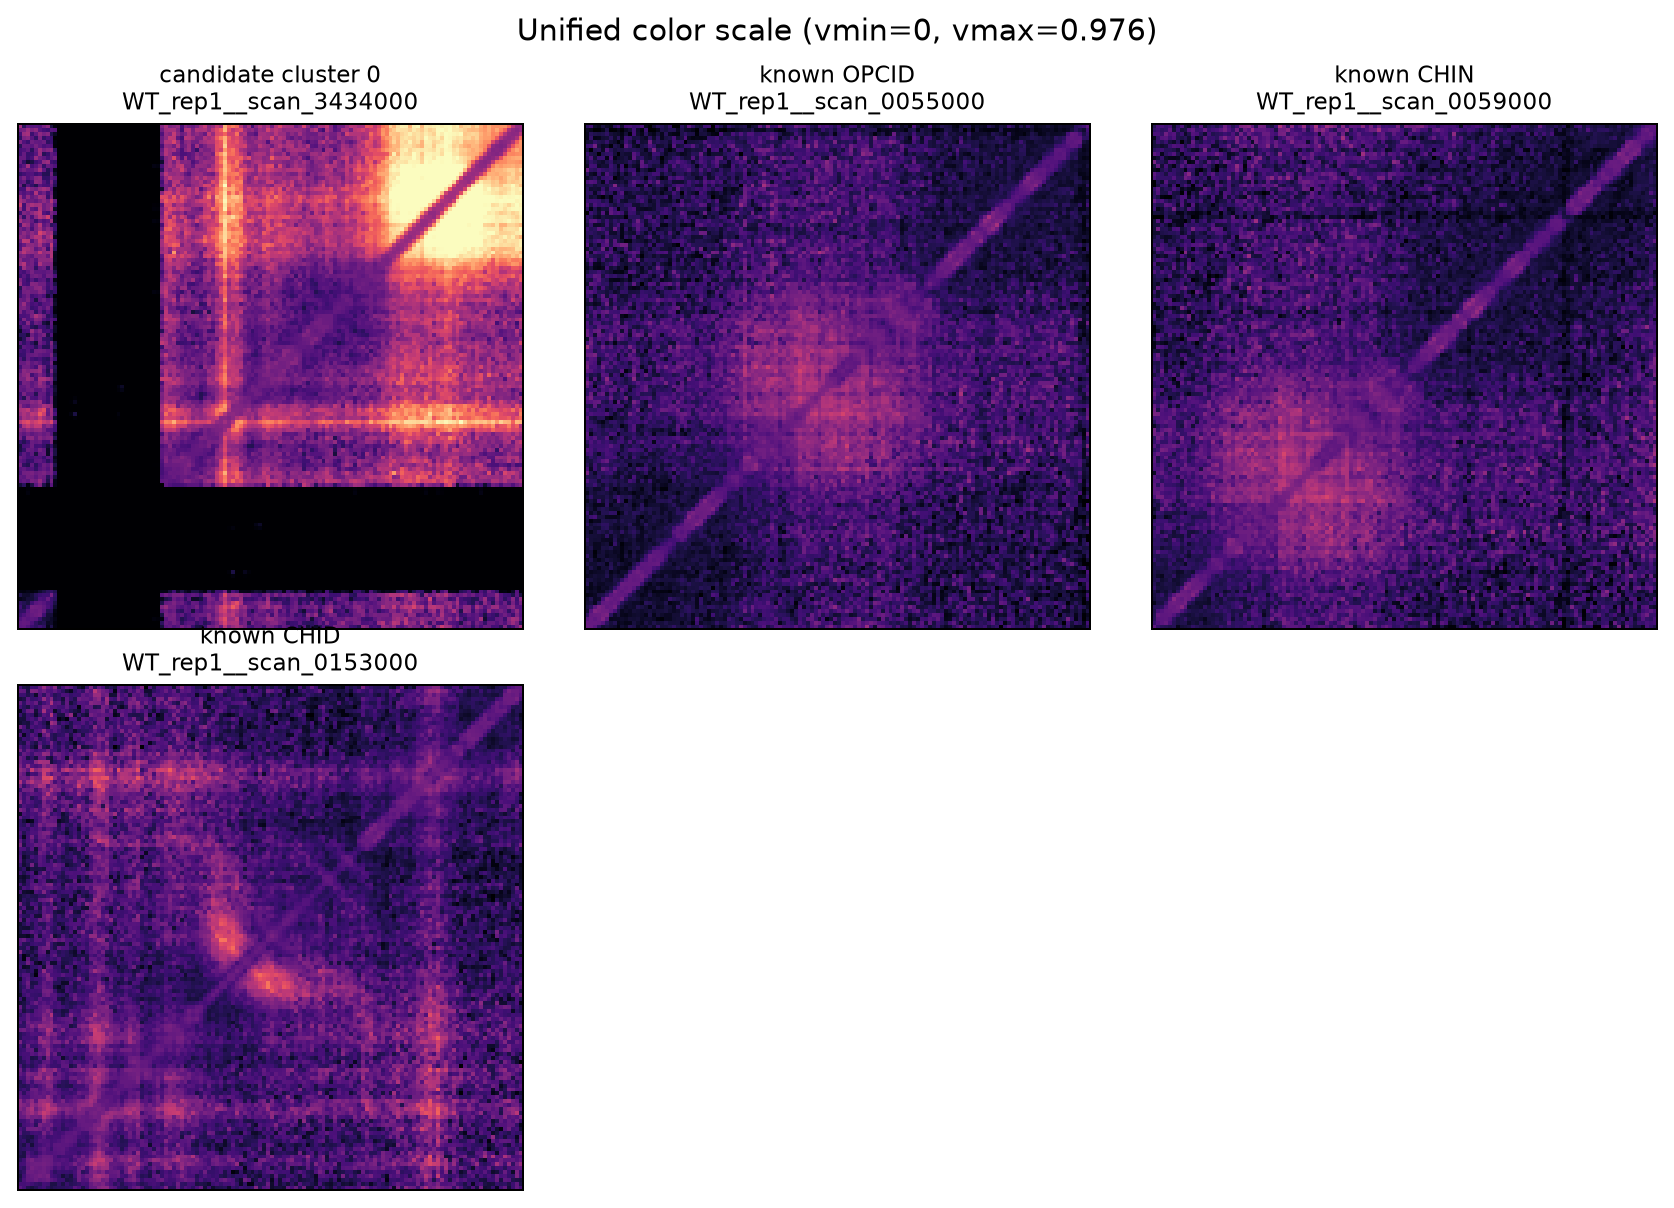
\includegraphics[width=\linewidth]{../results/clustering/cluster_representatives.png}\\[0.3em]
\scriptsize 灰色区域为数据缺口，不参与训练或打分。
\end{column}
\begin{column}{0.54\textwidth}
\begin{lstlisting}[basicstyle=\ttfamily\scriptsize]
valid_counts = window_mask.sum(dim=(1, 2))
squared_error = (prediction - target).square()[:, 0]
per_window = (squared_error * window_mask).sum(dim=(1, 2)) / valid_counts
\end{lstlisting}
\small
调用方先取逐窗口有效 mask 与上三角 mask 的交集，再传入
\texttt{masked\_mse}。每个窗口使用独立分母，避免缺口比例改变候选排序。
\end{column}
\end{columns}

\vspace{0.5em}
\small\textbf{结果检查：}误差与接触强度 Pearson 相关为 0.828；高分明显受强度影响，不能直接解释为新结构。
\end{frame}

\begin{frame}{候选聚类与独立位置}
\begin{columns}[T,onlytextwidth]
\begin{column}{0.64\textwidth}
\centering
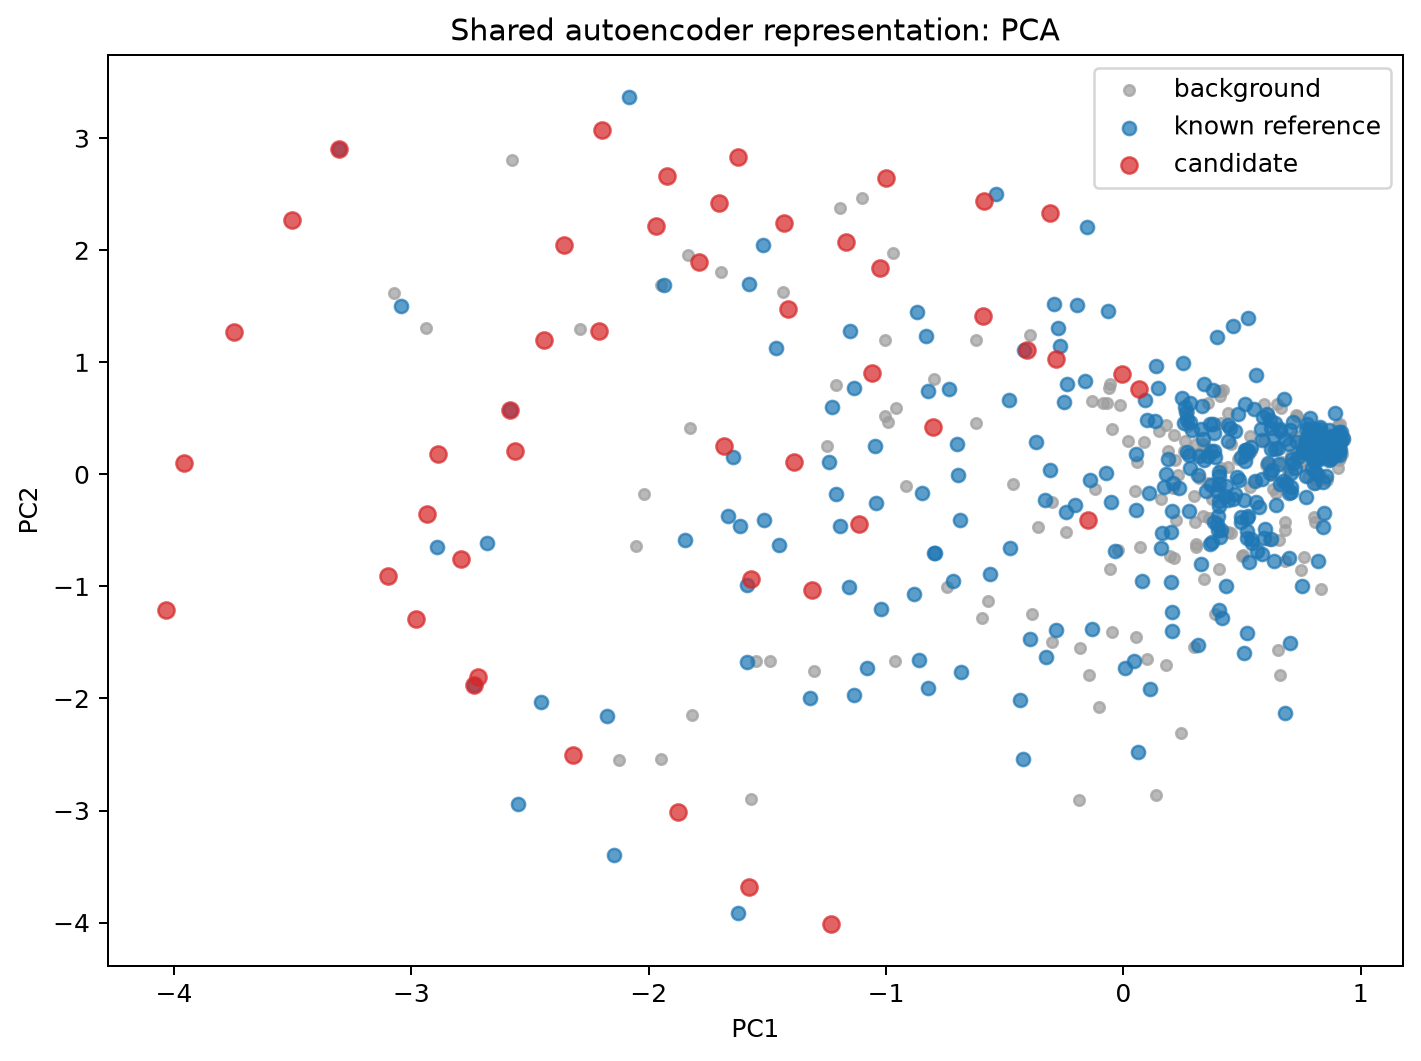
\includegraphics[height=0.60\textheight,keepaspectratio]{../results/clustering/pca_groups.png}\\[0.2em]
\scriptsize 图中显示前两个主成分；DBSCAN 实际使用 10 维白化 PCA 坐标。
\end{column}
\begin{column}{0.32\textwidth}
\small
\textbf{47 个候选窗口}\\[0.3em]
$\downarrow$ 合并重叠窗口\\[0.3em]
\textbf{10 个独立位置}

\vspace{0.8em}
唯一非噪声簇包含：
\begin{itemize}
\item 297 个已知参考
\item 9 个候选窗口
\item 4 个独立候选位置
\end{itemize}
\end{column}
\end{columns}

\vspace{0.4em}
\small\textbf{结论：}没有簇同时满足“至少 5 个独立位置、无已知参考、候选不与已知结构重叠”，本次不宣称发现新结构。
\end{frame}

\begin{frame}{三条件全基因组轨道}
\centering
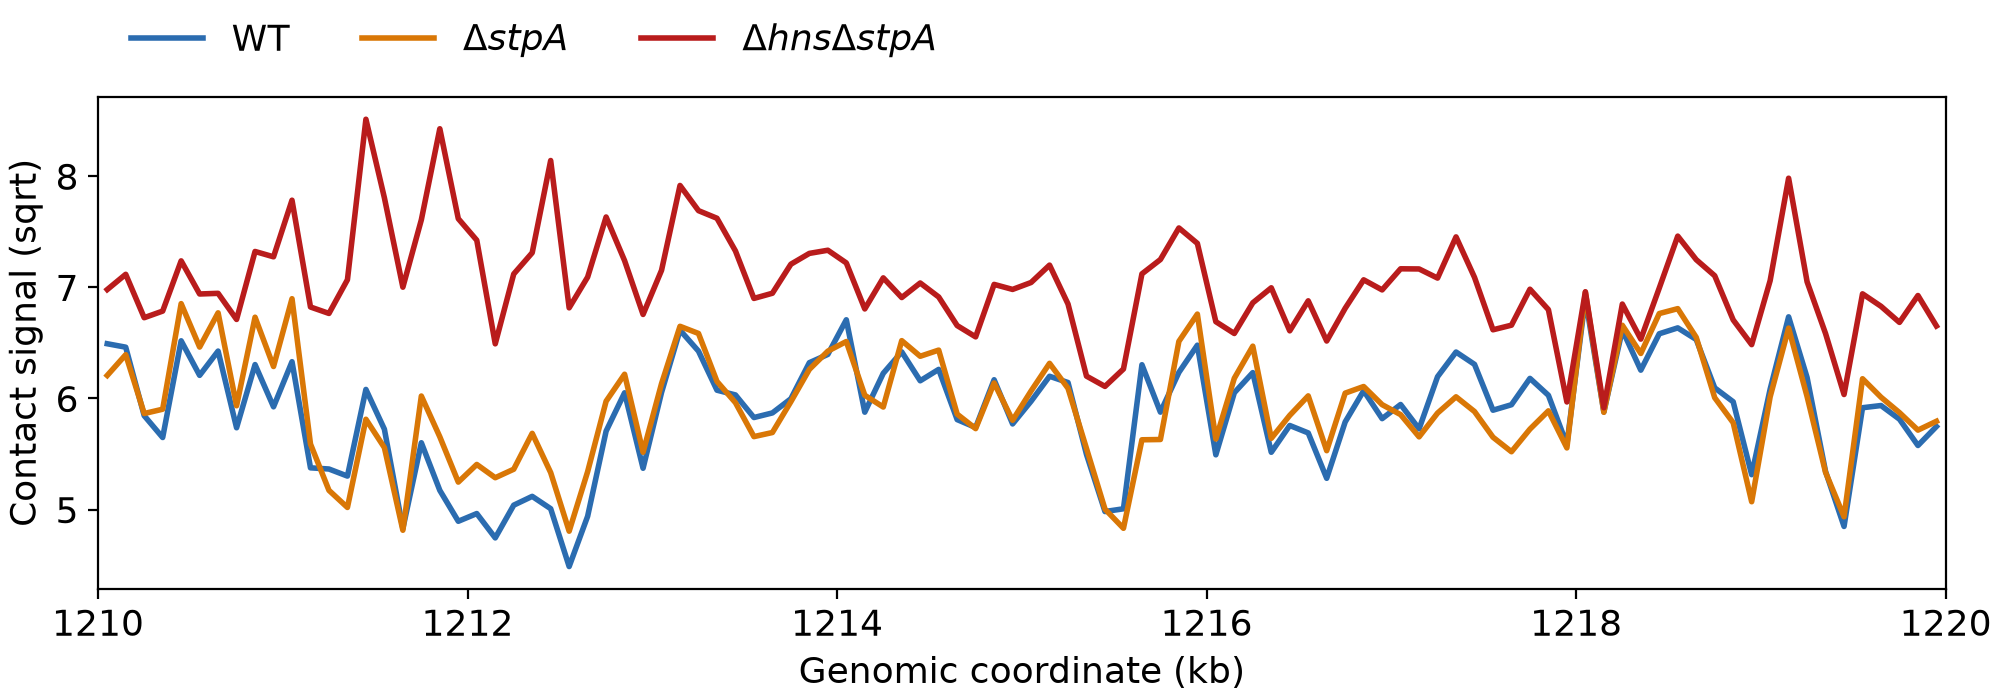
\includegraphics[width=0.98\textwidth]{../results/tracks/tracks_1210000_1220000_slide.png}\\[0.3em]

\raggedright\small
放大展示 1,210,000--1,220,000 bp 的条件均值；完整四面板见报告。\\[0.35em]
每个重复先按总接触量归一化；在线性尺度平均，再开平方显示。\\[0.35em]
全基因组连续输出 \textbf{465 张}四面板图，末图覆盖到 4,641,652 bp。\\[0.35em]
\textcolor{projectblue}{轨道用于定位和展示局部差异；曲线高低不等于统计显著性。}
\end{frame}
